\large

%In the future there will be used more wireless sensor networks  to different task and many nodes in these networks, can be placed at low heights, where communication between nodes get worse, as the path loss (PL) increases as the multipath waves can no longer be ignored. This will effect the link budget, when designing the antennas.

In the future wireless sensor networks will be more common and a problem related to this is the placement of the antennas. In many cases the antennas might be placed relatively low and this complicates calculations of the path loss (PL) as different propagation methods becomes significant. 

\begin{center}
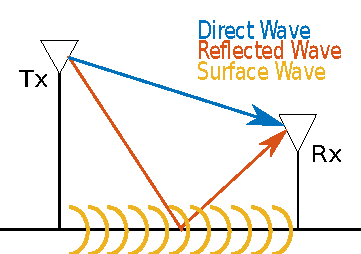
\includegraphics[scale=0.75]{pix/poster_cropped.pdf}
\captionof{figure}{Different propagation methods.}
\label{fig:name}
\end{center}
